
\documentclass[submit]{harvardml}

% Put in your full name and email address.
\name{Timothy Kang}
\email{tkang01@fas.harvard.edu}

% List any people you worked with.
\collaborators{%
  Jeff Chang
}

% You don't need to change these.
\course{CS181-S16}
\assignment{Assignment \#3}
\duedate{5:00pm March 25, 2016}

\usepackage[OT1]{fontenc}
\usepackage[colorlinks,citecolor=blue,urlcolor=blue]{hyperref}
\usepackage[pdftex]{graphicx}
\usepackage{subfig}
\usepackage{fullpage}
\usepackage{palatino}
\usepackage{mathpazo}
\usepackage{amsmath}
\usepackage{amssymb}
\usepackage{color}
\usepackage{todonotes}
\usepackage{listings}
\usepackage{common}
\usepackage{bm}
\newcommand{\mbf}[1]{\mathbf{#1}}
\usepackage[mmddyyyy,hhmmss]{datetime}

\definecolor{verbgray}{gray}{0.9}

\lstnewenvironment{csv}{%
  \lstset{backgroundcolor=\color{verbgray},
  frame=single,
  framerule=0pt,
  basicstyle=\ttfamily,
  columns=fullflexible}}{}

\begin{document}
\begin{center}
{\Large Homework 3: SVM}\\
\end{center}

There is a mathematical component and a programming component to this homework.
Please submit ONLY your PDF to Canvas, and push all of your work to your Github
repository. If a question asks you to make any plots, like Problem 3, please
include those in the writeup.

%%%%%%%%%%%%%%%%%%%%%%%%%%%%%%%%%%%%%%%%%%%%%
% Problem 1
%%%%%%%%%%%%%%%%%%%%%%%%%%%%%%%%%%%%%%%%%%%%%
\begin{problem}[Fitting an SVM by hand, 8pts]
Consider a dataset with the following 6 points in $1D$: \[\{(x_1, y_1)\} =\{(-3
, +1 ), (-2 , +1 ) , (-1,  -1 ), ( 1 , -1 ), ( 2 , +1 ), ( 3 , +1 )\}\] Consider
mapping these points to $2$ dimensions using the feature vector $\phi : x
\mapsto (x, x^2)$. The max-margin classifier objective is given by:
\begin{equation}
  \min_{\mathbf{w}, w_0} \|\mathbf{w}\|_2^2 \quad \text{s.t.} \quad y_i(\mathbf{w}^T \phi(x_i) +
  w_0) \geq 1,~\forall i
\end{equation}

Note: the purpose of this exercise is to solve the SVM without the help of a
computer, relying instead on principled rules and properties of these
classifiers. The exercise has been broken down into a series of questions, each
providing a part of the solution. Make sure to follow the logical structure of
the exercise when composing your answer and to justify each step.

\begin{enumerate}
  \item Write down a vector that is parallel to the optimal vector $\mathbf{w}$. Justify
    your answer.
  \item What is the value of the margin achieved by $\mathbf{w}$? Justify your
    answer.
  \item Solve for $\mathbf{w}$ using your answers to the two previous questions.
  \item Solve for $w_0$. Justify your answer.
  \item Write down the discriminant as an explicit function of $x$.
\end{enumerate}

\end{problem}
\subsection*{Solution}
\begin{enumerate}
	\item We begin by recognizing that $\mathbf{w}$ is perpendicular to the hyperplane. Given two points
		\textbf{on} the hyperplane $\mathbf{x_1}$ and $\mathbf{x_2}$, we have 
			$$\mathbf{w}^T(\phi(x_1) - \phi(x_2)) = w_0 - w_0 = 0$$
		From this, we know that any vector that is parallel to $\mathbf{w}$ will be perpendicular to the 
		hyperplane. The plot generated using the basis function $\phi: x \mapsto(x,x^2)$ is as following\\ \\
			\centerline{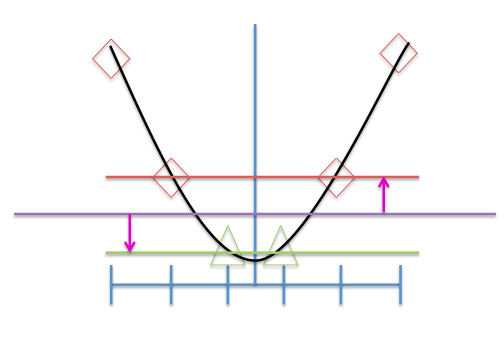
\includegraphics[scale=0.3]{./ayy}}
		where the diamonds represent the class +1 and the triangles represent the class -1. Because we used 
		a quadratic basis function with one dimensional points, the lines connecting the support vectors are 
		clearly the horizontal lines	at $ y = 4$ and $y = 1$. If we use the fact that, at the support vectors, 
		$y_i(\mathbf{w}^T\phi(x_i) + w_0) = 1$, 
		then the distance from a point on each line connecting the support vectors to the hyperplane is given by 
			$$ r = \frac{y_i(\mathbf{w}^T\phi(x_i) + w_0)}{\| \mathbf{w} \|_2}$$
		because the numerator is 1 for both support vectors, we know that the distance from a support vector 
		at $y = 4$ to the hyperplane must equal the distance from a support vector at $y = 1$ to the hyperplane.
		The hyperplane would also be a horizontal line, which maximizes the margin, at $y = 2.5$. Therefore, 
		a vector that is parallel to $\mathbf{w}$ is literally any vector that is perpendicular to the hyperplane, such 
		as $\left[0 \text{      {} } 1\right]$
	\item Using most of the argument from above, we know that the distance between each support vector 
		and the hyperplane must be the same. Therefore, because the distance between the support vectors 
		is 3, the margin from one support vector to the hyperplane is 1.5.
	\item Again, because $y_i(\mathbf{w}^T\phi(x_i) + w_0) = 1$ at the support vectors, we have that 
		$$ r = \frac{1}{\|\mathbf{w}\|_2}$$
		where $r$ is the distance from the support vector to the hyperplane. However, because we already established 
		that $r = 1.5$ in the previous question, we know that this is only possible if 
			$$\|\mathbf{w}\|_2 = \frac{2}{3}$$
		Now, if we use the fact that parallel vectors are multiples of each other, we can rewrite this as 
			$$\| \left[0 \text{      {} } 1\right] \cdot c\|_2 = \frac{2}{3}$$	
		where $c$ is some multiplicative constant, which yields that $c = \frac{2}{3}$, or 
			$$\mathbf{w} = \left[0 \text{      {} }  \frac{2}{3}\right]$$	
	\item To solve for $w_0$, we make use of the fact that $\mathbf{w} = \left[0, 1\right]\cdot c$, where $c$ is some
		multiplicative constant. Plugging this into our discriminant function, we have 
			$$y_i[\left[0 \text{      {} } 1\right] \cdot c \cdot \phi(x_i) + w_i] = 1$$
		for the support vectors. Using one point from each support vector, hence each class, we have the 
		system of equations
			\begin{align*}
				1 \cdot [\left[0 \text{      {} } 1\right] \cdot c \cdot \left[2 \text{      {} } 4\right]+ w_i] = 1 &\implies 4c + w_0 = 1\\
				-1 \cdot [\left[0 \text{      {} } 1\right] \cdot c \cdot \left[-1 \text{      {} } 1\right]+ w_i] = 1 & \implies -c -w_0 = 1
			\end{align*}
		rearranging the equations and setting $c$ equal to each other yields 
			$$w_0 = -\frac{5}{3}$$
	\item To find the discriminant as an explicit function of $x$, we simply plug in the values of $\mathbf{w}$ and 
		$w_0$ that we found above
			\begin{align*}
				f(x) &= \left[0 \text{      {} }  \frac{2}{3}\right]^T [x \text{      {} }  x^2] - \frac{5}{3} \\ 
				&= \frac{2}{3}x^2 - \frac{5}{3}
			\end{align*}
		If we plug in $x = 2$, we get back +1, and if we plug in $x = -1$, we get back -1, which corresponds to 
		our support vectors/classes. 
\end{enumerate}


\newpage
%%%%%%%%%%%%%%%%%%%%%%%%%%%%%%%%%%%%%%%%%%%%%
% Problem 2
%%%%%%%%%%%%%%%%%%%%%%%%%%%%%%%%%%%%%%%%%%%%%
\begin{problem}[Composing Kernel Functions , 7pts]
Prove that
\begin{align*}
	K(\boldx, \boldx') &= \exp\{ -||\boldx - \boldx'||^2_2 \}\,,
\end{align*}
where~$\boldx,\boldx'\in\reals^D$ is a valid kernel, using only the following
properties.  If~$K_1(\cdot,\cdot)$ and~$K_2(\cdot,\cdot)$ are valid kernels,
then the following are also valid kernels:
\begin{align*}
	K(\boldx, \boldx') &= c\,K_1(\boldx, \boldx') \quad \text{for $c>0$}\\
	K(\boldx, \boldx') &= K_1(\boldx, \boldx') + K_2(\boldx, \boldx')\\
	K(\boldx, \boldx') &= K_1(\boldx, \boldx')\,K_2(\boldx, \boldx')\\
	K(\boldx, \boldx') &= \exp\{ K_1(\boldx, \boldx') \}\\
  K(\boldx, \boldx') &= f(\boldx)\,K_1(\boldx, \boldx')\,f(\boldx') \quad
  \text{where $f$ is any function from~$\reals^D$ to $\reals$}
\end{align*}

 \end{problem}
\subsection*{Solution}

We begin by first expanding the square to get 
	$$-  \mathbf{x}^T\mathbf{x} - (\mathbf{x'})^T\mathbf{x'} + 2 \mathbf{x}^T\mathbf{x'}$$
which allows us to rewrite the expression for the kernel as 
	$$\text{exp}\left\{-  \mathbf{x}^T\mathbf{x} - (\mathbf{x'})^T\mathbf{x'} + 2 \mathbf{x}^T\mathbf{x'}\right\} = 
	\text{exp} \left\{-  \mathbf{x}^T\mathbf{x} \right\}\text{exp} \left\{2 \mathbf{x}^T\mathbf{x'}\right\} \text{exp} \left\{
	- (\mathbf{x'})^T\mathbf{x'}   \right\}$$
We know that $\mathbf{x}^T\mathbf{x}$ is just the linear kernel, whose validity is trivial to show. Combining this 
with the fourth and fifth property shows that this is a valid kernel. Specifically, the middle term is the valid linear kernel
multiplied by some positive constant (first property) with the exponential function applied to it (fourth property). The 
outer terms are simply applying the same function to $\mathbf{x}$ and $\mathbf{x'}$, where the function 
returns the dot product of the input and itself and applies the exponential function to the negation of the product.\\ \\
I accidentally misread the problem and thought we were supposed to prove the five properties, so I did that. And because I spent like 2 hours doing that, I figured I might as well include it in the submission. \\ \\
We can prove that a kernel is positive by showing that it is positive semi-definite, or that $\forall \mathbf{y}: 
\mathbf{y}^T K(\mathbf{x}, \mathbf{x'}) \mathbf{y} \geq 0$
\begin{enumerate}
	\item 
		\begin{align*}
			K(\mathbf{x}, \mathbf{x'}) &= cK_1 (\mathbf{x},\mathbf{x'}) \\
			\implies \mathbf{y}^T K(\mathbf{x}, \mathbf{x'})\mathbf{y} &= \mathbf{y}^T cK_1 (\mathbf{x},
			\mathbf{x'}) \mathbf{y}\\ 
			&= c  \left[\mathbf{y}^T K_1 (\mathbf{x},\mathbf{x'}) \mathbf{y}\right] \geq 0 
		\end{align*}
		Because $K_1$ is a valid kernel, we know that it is positive semi-definite, and multiplying it by a 
		positive constant $c$ will result in a positive semi-definite output. Therefore, $K$ is a valid kernel 
		because it is positive semi-definite.
	\item We can generalize this kernel to 
			$$ K(\mbf{x}, \mbf{x'}) = \alpha K_1 (\mbf{x}, \mbf{x'}) + \beta K_2(\mbf{x}, \mbf{x'})$$
		where  $\alpha, \beta > 0$ (in the case of this property, $\alpha = \beta = 1$). 
		\begin{align*}
			\mbf{y}^TK(\mbf{x},\mbf{x'})\mbf{y} &= \mbf{y}^T \left[ \alpha K_1 (\mbf{x}, \mbf{x'}) + \beta 
			K_2(\mbf{x}, \mbf{x'}) \right] \mbf{y} \\ 
			&= \mbf{y}^T \alpha K_1 \mbf{y} + \mbf{y}^T \beta K_2 + \mbf{y} \\
			&= \alpha \mbf{y}^T K_1 (\mbf{x}, \mbf{x'}) \mbf{y} + \beta \mbf{y}^T K_2(\mbf{x}, \mbf{x'}) \mbf{y} \geq 0
		\end{align*}
		We know that this equality is true because $K_1, K_2$ are valid kernels (hence, $\mbf{y}^T K_i \mbf{y} \geq 0$)
		and the product of a valid kernel and a positive constant is a valid kernel, as shown above. Therefore, 
		$K(\boldx, \boldx') = K_1(\boldx, \boldx') + K_2(\boldx, \boldx')$ is a valid kernel.
	\item If we consider the Gram matrix $K$, we realize that it is simply a Hadamard product $K_1 \circ K_2$. Next, 
		we use the fact that the kernel is a covariance function, implying that $K_1$ and $K_2$ are covariance matrices 
		(for $K_{1i}$ and $K_{2i}$, respectively). We prove that covariance matrices are positive semi-definite:
		\begin{align*}
			\mbf{y}^T \mbf{C} \mbf{y} &= \mbf{y}^T E\left[(\mbf{x} - \mbf{x'})(\mbf{x} - \mbf{x'})^T  \right] \mbf{y} \\
			&= E\left [\mbf{y}^T (\mbf{x} - \mbf{x'})(\mbf{x} - \mbf{x'})^T \mbf{y}\right] \\
			&= \sigma^2
		\end{align*}
		This comes from the fact that $\sigma = \mbf{y}^T (\mbf{x} - \mbf{x'})$ or $(\mbf{x} -\mbf{x'})^T \mbf{y}$. \\ \\
		Using the Schur product theorem, we know that the Hadamard product of two positive definite matrices is also 
		positive definite (positive definiteness is a stricter condition than positive semi-definiteness). Therefore, 
		with $K_1(\mbf{x},\mbf{x'})K_2(\mbf{x},\mbf{x'})$, we have the Hadamard product of two covariance 
		matrices, which yields a positive semi-definite matrix. Therefore, this is a valid kernel.
	\item 
		\begin{align*}
			\mbf{y}^T K(\mbf{x},\mbf{x'}) \mbf{y} &= \mbf{y}^T e^{K_1(\mbf{x},\mbf{x'})} \mbf{y} \\
			&= (\ln \mbf{y}^T) K_1(\mbf{x},\mbf{x'}) (\ln \mbf{y})
		\end{align*}
		Since the condition for positive semi-definiteness is defined $\forall y$, we still have that 
			$$\mbf{y}^T K_1(\mbf{x},\mbf{x'}) \mbf{y} \geq 0$$
		Therefore, $K$ is a valid kernel.	\\ \\
		Alternatively, suppose $K_1$ is a valid kernel. Then,
			$$K(\mbf{x}, \mbf{x'}) = f(K_1(\mbf{x},\mbf{x'}))$$
		where $f$ is a polynomial with positive coefficients, is a valid kernel. We know this because each term 
		is a product of kernels with positive coefficients	(combine properties two and three).Next, if we 
		recall the Taylor series expansion for $e^x = 1 + x + \frac{x^2}{2} + \dots + \frac{x^i}{i!}$, we see 
		that property four is a valid kernel.
	\item 
		\begin{align*}
			f(\mbf{x}) K_1(\mbf{x},\mbf{x'}) f(\mbf{x'}) &= f(\mbf{x}) f(\mbf{x'}) K_1(\mbf{x},\mbf{x'}) \\
			&= f(\mbf{x}) f(\mbf{x'}) \left<\phi(\mbf{x}), \phi(\mbf{x'}) \right>\\
			&=  \left<f(\mbf{x}) \phi(\mbf{x}), f(\mbf{x'}) \phi(\mbf{x'}) \right>\\
			&= \left<\phi' (\mbf{x}), \phi'(\mbf{x'}) \right>
		\end{align*}
		Therefore, this is a valid kernel.
\end{enumerate}


\newpage
%%%%%%%%%%%%%%%%%%%%%%%%%%%%%%%%%%%%%%%%%%%%%
% Problem 3
%%%%%%%%%%%%%%%%%%%%%%%%%%%%%%%%%%%%%%%%%%%%%
\begin{problem}[Scaling up your SVM solver, 10pts (+7pts with extra credit)]



In the previous homework, you studied a simple data set of fruit measurements.
We would like you to code up a few simple SVM solvers to classify lemons from
apples. To do this, read the paper at
\url{http://www.jmlr.org/papers/volume6/bordes05a/bordes05a.pdf} and implement
the Kernel Perceptron algorithm and the Budget Kernel Perceptron algorithm. The provided code has a base Perceptron class, which you will inherit to write KernelPerceptron and BudgetKernelPerceptron. This has been set up for you in problem3.py. The provided data is linearly separable. Make the optimization as fast as
possible. 

Additionally, we would like you to do some experimentation with the hyperparameters for each of these models. Try seeing if you can identify some patterns by changing $\beta$, N (maximum number of support vectors), or the number of random samples you take.  Note the training time, accuracy,  shapes/orientations of hyperplanes, and number of support vectors for various setups. We are intentionally leaving this open-ended to allow for experimentation, and so we will be looking for your thought process and not a rigid graph this time. That being said, any visualizations that you want us to grade and refer to in your descriptions should be included in this writeup. You can use the trivial $K(\mathbf{x_1}, \mathbf{x_2}) = \mathbf{x_1}^T\mathbf{x_2}$ kernel for this problem, though you are welcome to experiment with more interesting kernels too. Also, answer the following reading questions in one or two sentences each.

\begin{enumerate}
\item In one short sentence, state the main purpose of the paper?
\item Identify each of the parameters in Eq. 1
\item State one guarantee for the Kernel perceptron algorithm described in the
  paper.
\item What is the main way the budget kernel perceptron algorithm tries to
  improve on the perceptron algorithm.
\item In simple words, what is the theoretical guarantee of LASVM algorithm? How
  does it compare to its practical performance?
\end{enumerate}


For extra credit (+7 pts), implement the SMO algorithm and implement the LASVM process and do the same as above.


\end{problem}

\subsection*{Solution}
\begin{enumerate}
	\item The paper elaborates on current methods of classification involving support vector machines, proposes
		a new algorithm - an online SVM algorithm called LAVSM - and analyzes its performance relative to 
		other algorithms with respect to various parameters. 
	\item Equation 1:
		$$\hat{y}(x) = w'\phi(x) + b$$
		$w$ is a weight vector that is found by running a fit function on training data. $b$ is a bias parameter 
		that is determined before or during runtime, depending on the algorithm (kernel perceptron 
		and budget kernel perceptron both specify $b = 0$ in this paper). Finally, $\phi(x)$ is a basis function
		that transforms the inputs into feature vectors, which is done using kernel functions. 
	\item The Kernel perceptron algorithm guarantees that it will converge with a finite number of support vectors and 
		that a point will not be misclassified more than once - after the first incident, it gets added to the support 
		vectors. 
	\item The budget kernel algorithm places an upper bound on how many support vectors there can be, which
		can reduce runtime significantly, depending on what kernel function is used. This reduces computational
		resources that are spent and helps avoid potential overfitting. 
	\item LASVM converges to the known SVM solution, matches the SVM accuracy after a single sequential iteration,
		and is capable of handling noisy data. Also, it guarantees that it will reach at $\tau$-approximate solution - one
		with tolerance of $\tau$ (theorem 18). 
\end{enumerate}

\noindent\textbf{Preliminaries} \\ 
\textbf{Specs:} I used a 2014 Macbook Air with 4 GB of RAM.  \\ 
After reading the paper and deciphering the pseudocode for the perceptron algorithms, I knew that my first step would be to decide which kernel functions I wanted to use. Naturally, due to the triviality associated with implementing it, I choose the linear kernel to be my starting point, which I aptly titled \texttt{trivial\_kernel}. I decided that, after running my code using \texttt{trivial\_kernel}, it would make sense to run it using a nontrivial kernel, such as the Gaussian or RBF kernel, which I denoted as \texttt{nontrivial\_kernel}. I chose the RBF kernel for the simplicity of implementation and because the return value of the Gaussian kernel decreases with distance between vectors, so it would serve as a relatively accurate similarity measure. Finally, to be completely thorough, I decided to make a ``stupid" kernel, which consisted of multiplying the output of \texttt{trivial\_kernel} and \texttt{nontrivial\_kernel}; this is a valid kernel since I am simply multiplying two valid kernels - I refer to problem 2 for the proof of this. \\ \\
Furthermore, I interpreted the phrase ``random example/sample" in the pseudocode to mean that the data points that I used for the fit function should be randomized. Therefore, I wrote a function that would shuffle all of the data and 
preserve the ``pairing" between the $X$ and $Y$ values (that is, I shuffled the three column data frame in its entirety and then split it back up into $X$ and $Y$). \\ \\
Once I finished successfully implementing the kernel perceptron and the budget kernel perceptron algorithms, I noticed that the plots produced by the two algorithms (and the SMO and LASVM algorithms) were similar if not identical to the following - this made sense, since I randomize the inputs everytime. \\ \\
	\centerline{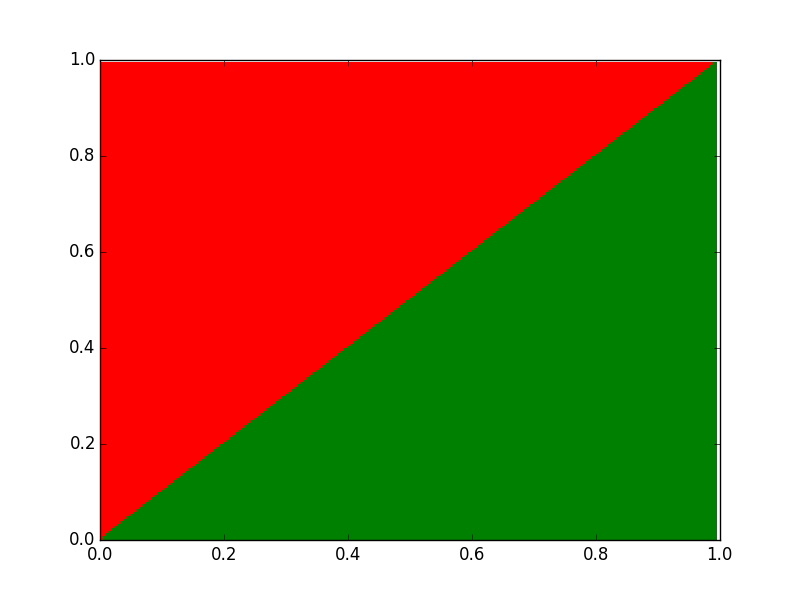
\includegraphics[scale = 0.5]{./k}}
As such, I will not be including any more plots of the classifications in the rest of this write-up, as they will not yield any new or useful information. From this point on, I ran a script that tested how long it took to fit the data and ran cross-validation using a 60-40 split. I kept \texttt{numsamples} at 20000 for both the kernel perceptron and budget kernel perceptron algorithms but changed which kernel was used and the parameters for the budget kernel perceptron.\\ \\
\noindent\textbf{Data: Timing} \\
I began by running my timing script on the budget kernel perceptron algorithm, since I assumed that it would run faster for the reasons listed above, and ran 10, 50, and 100 iterations using each of the kernels and the following parameters: $\beta = 0, N = 100, \text{numsamples} = 20000$. When I did the same for the kernel perceptron algorithm, it would take upwards of 20 minutes to run 10 iterations of the timing script using the Gaussian kernel or the stupid kernel, so in an effort to save time and increase overall productivity, I decided to only do 10 iterations. The csv's generated by the script can be found in \texttt{bk\_times} and \texttt{sk\_times}, where sk means simple kernel.

\begin{table}[htb]
\centering
\caption{Runtimes of SK and BK algorithms using different kernels}
\label{my-label}
\begin{tabular}{l|llllll}
        & BK Linear & SK Linear & BK RBF & SK RBF  & BK Stupid & SK Stupid \\ \hline
1       & 10.488    & 25.677    & 16.447 & 130.849 & 46.505    & 94.750    \\
2       & 9.673     & 19.453    & 16.176 & 123,717 & 41.282    & 80.652    \\
3       & 9.801     & 14.742    & 16.362 & 157.132 & 38.367    & 100.298   \\
4       & 10.615    & 1.024     & 15.698 & 150.990 & 39.917    & 80.396    \\
5       & 10.732    & 21.358    & 16.113 & 137.577 & 37.236    & 82.975    \\
6       & 9.552     & 13.979    & 17.261 & 83.161  & 41.422    & 82.234    \\
7       & 9.702     & 11.992    & 15.660 & 104.138 & 41.387    & 85.943    \\
8       & 9.572     & 9.699     & 17.966 & 121.531 & 38.097    & 94.700    \\
9       & 9.678     & 8.344     & 15.944 & 114.237 & 38.327    & 90.182    \\
10      & 6.261     & 25.311    & 16.731 & 124.860 & 40.328    & 87.509    \\ \hline
Average & 9.607     & 15.159    & 16.436 & 124.820 & 40.287    & 87.964   
\end{tabular}
\end{table}
\noindent It was clear that the budget kernel perceptron algorithm ran significantly faster than the basic kernel perceptron algorithm, which makes sense since the budget kernel perceptron has an upper limit to how many support vectors it stored - in this case 100. Out of curiosity, I decided to measure how many support vectors the basic kernel perceptron stored. Because I was short on time, I only ran five iterations. 
\begin{table}[hbt]
\centering
\caption{Number of support vectors using SK algorithms with different kernels}
\label{my-label}
\begin{tabular}{l|lll}
        & SK Linear & SK RBF & SK Stupid \\ \hline
1       & 311       & 542    & 361       \\
2       & 252       & 504    & 401       \\
3       & 307       & 574    & 368       \\
4       & 105       & 586    & 327       \\
5       & 157       & 512    & 403       \\ \hline
Average & 226.4     & 543.6  & 372      
\end{tabular}
\end{table}

\noindent Given the fact that the budget kernel perceptron algorithm could only have 100 support vectors maximum, it makes sense why the runtime for the budget kernel algorithm was significantly better than that of the simple kernel perceptron algorithm. Because both perceptron algorithms require iterating over the entirety of the support vectors during the training phase, having to deal with over 500 support vectors would be slightly less than optimal. \\ \\ 
Once I had generated the data sets above, I decided to mess with the parameters related to the budget kernel perceptron algorithm to see how it would effect runtime. I hypothesized that runtime as a function of $N$, or the maximum number of support vectors, was monotonic, based on the comparison of the SK and BK algorithms' runtimes. Therefore, I decreased $N$. Given that $\beta$ represents a ``mistake threshold", for lack of a better term, I assumed that increasing the value of $\beta$ would increase run time as the perceptron would be stricter - more things will be classified as mistakes. I ran 10 iterations of the timing script. \\ \\ \\ \\ \\
\begin{table}[hbt]
\centering
\caption{Runtimes of BK algorithm, keeping numsamples and $\beta$ constant but reducing $N$ to 50}
\label{my-label}
\begin{tabular}{l|lll}
        & BK Linear & BK RBF & BK Stupid \\ \hline
1       & 6.089     & 16.907 & 19.996    \\
2       & 6.911     & 15.922 & 19.630    \\
3       & 7.317     & 16.917 & 22.445    \\
4       & 5.475     & 17.025 & 20.251    \\
5       & 6.829     & 16.133 & 20.251    \\
6       & 3.687     & 16.907 & 19.120    \\
7       & 6.643     & 17.235 & 24.059    \\
8       & 8.609     & 17.181 & 18.634    \\
9       & 7.845     & 16.591 & 18.389    \\
10      & 6.652     & 17.05  & 18.773    \\ \hline
Average & 6.605     & 15.852 & 20.063   
\end{tabular}
\end{table}

\noindent As was expected, the average run time for each kernel function decreased by a nontrivial amount after decreasing the maximum number of support vectors. Intuitively, this makes sense since we halved the number of support vectors, which is significant given the fact that we iterate over \textbf{all} of the support vectors at each iteration of the perceptron. 
\begin{table}[hbt]
\centering
\caption{Runtimes of BK algorithm, keeping numsamples and $N$ constant but increasing $\beta$ to 0.5}
\label{my-label}
\begin{tabular}{l|lll}
        & BK Linear & BK RBF & BK Stupid \\ \hline
1       & 12.392    & 18.993 & 24.736    \\
2       & 12.070    & 19.576 & 24.509    \\
3       & 15.322    & 21.390 & 26.699    \\
4       & 12.705    & 21.577 & 26.549    \\
5       & 11.137    & 22.301 & 23.328    \\
6       & 11.347    & 22.683 & 23.453    \\
7       & 9.843     & 23.235 & 23.415    \\
8       & 11.097    & 19.407 & 22.214    \\
9       & 10.715    & 25.131 & 22.231    \\
10      & 13.725    & 25.694 & 23.821    \\ \hline
Average & 12.035    & 22.053 & 24.095   
\end{tabular}
\end{table}
\noindent For the linear and RBF kernel, average run time increased. However, the stupid kernel's average run time decreased by a relatively significant amount. This made some sense, since the stupid kernel is just the product of the linear and RBF kernel, which means that, assuming that both values are positive or negative, the kernel function would return a higher value than if I had just used the linear or RBF kernel. This is significant because we check to see if the product of $\hat{y}$ and $y$ is less than $\beta$, which we have just increased. Therefore, we would do the ``updating" step (appending indices to the support array, removing elements from the support array, etc.) a fewer number of times. \\ \\ 
I never ran my timing script with different values for numsample, mainly because it was fairly obvious what would happen: decreasing numsample would decrease runtime, since we iterate the fit function however many times numsample specifies.\\ \\
\textbf{Data: Accuracy}
With timing data collected, I moved on to checking the accuracy of each algorithm. To do so, I ran cross-validation using a 60-40 split on the data, after shuffling it using the aforementioned shuffle function. The split itself was done using \texttt{cross\_validation.train\_test\_split} from the \texttt{sklearn} library. As with before, I first ran cross-validation on the budget kernel and simple kernel perceptron algorithm using the three different kernel functions and the following parameters: numsamples = 20000, $\beta = 0$, $N = 100$. 
\begin{table}[hbt]
\centering
\caption{Accuracy of SK and BK algorithms using different kernels}
\label{my-label}
\begin{tabular}{l|llllll}
        & BK Linear & SK Linear & BK RBF  & SK RBF  & BK Stupid & SK Stupid \\ \hline
1       & 99.94\%   & 99.95\%   & 98.95\% & 97.34\% & 99.50\%   & 99.78\%   \\
2       & 99.82\%   & 99.82\%   & 96.77\% & 97.25\% & 97.16\%   & 97.64\%   \\
3       & 99.12\%   & 99.94\%   & 97.92\% & 99.39\% & 97.83\%   & 99.40\%   \\
4       & 99.90\%   & 100\%     & 98.02\% & 99.58\% & 99.63\%   & 99.82\%   \\
5       & 100\%     & 100\%     & 98.36\% & 99.31\% & 96.31\%   & 99.87\%   \\ \hline
Average & 99.57\%   & 99.74\%   & 98.00\% & 98.57\% & 98.09\%   & 99.30\%  
\end{tabular}
\end{table}
Immediately, I noticed that across the board, the accuracy of budget kernel algorithm was slightly worse than that of the simple kernel algorithm, regardless of which kernel function was used. Intuitively, this made sense, since the budget kernel perceptron algorithm can only be at most as accurate as the simple kernel perceptron algorithm: the budget kernel algorithm does the same thing as the simple kernel algorithm with less support vectors. As such, what budget kernel has in computational advantage (speed and memory-wise), it loses in accuracy because it is essentially working with less data. \\ \\
As with the timing, I decided to check the accuracy of the budget kernel algorithm, holding numsamples constant and increasing and decreasing $N$ and $\beta$. 

\begin{table}[hbt]
\centering
\caption{Accuracy of BK algorithms, keeping numsamples and $\beta$ constant but reducing $N$ to 50}
\label{my-label}
\begin{tabular}{l|lll}
        & BK Linear & BK RBF  & BK Stupid \\ \hline
1       & 100\%     & 95.11\% & 95.72\%   \\
2       & 99.98\%   & 98.14\% & 96.99\%   \\
3       & 91.87\%   & 96.13\% & 95.05\%   \\
4       & 99.33\%   & 91.92\% & 99.33\%   \\
5       & 100\%     & 97.67\% & 97.56     \\ \hline
Average & 98.20\%   & 95.74\% & 96.93\%  
\end{tabular}
\end{table}
\noindent While the accuracy tests for this set certainly ran faster, the overall average accuracy was notably lower. Using the same logic above, this makes sense, since we're even further reducing the amount of data that is available for the training phase. 
\begin{table}[hbt]
\centering
\caption{Accuracy of BK algorithms, keeping numsamples and $\beta$ constant but reducing $N$ to 150}
\label{my-label}
\begin{tabular}{l|lll}
        & BK Linear & BK RBF  & BK Stupid \\ \hline
1       & 96.09\%   & 98.43\% & 99.46\%   \\
2       & 99.99\%   & 97.63\% & 98.96\%   \\
3       & 99.90\%   & 97.93\% & 94.37\%   \\
4       & 100\%     & 97.88\% & 99.70\%   \\
5       & 100\%     & 97.84\% & 99.27\%   \\ \hline
Average & 99.20\%   & 97.94\% & 98.35\%  
\end{tabular}
\end{table} \\
\noindent Overall, there wasn't a significant difference in the average accuracy when the maximum possible number of support vectors was increased. This was probably due to the fact that, by this point, the accuracy was nearing 100\% and random outlier values would heavily affect the mean, as was the case in this data set. \\ \\ \\\\ 
\begin{table}[hbt]
\centering
\caption{Accuracy of BK algorithms, keeping numsamples and $N$ constant but increasing $\beta$ to 0.5}
\label{my-label}
\begin{tabular}{l|lll}
        & BK Linear & BK RBF  & BK Stupid \\ \hline
1       & 99.94\%   & 99.14\% & 97.08\%   \\
2       & 91.39\%   & 92.44\% & 98.74\%   \\
3       & 99.97\%   & 97.38\% & 95.16\%   \\
4       & 97.39\%   & 98.84\% & 98.87\%   \\
5       & 98.62\%   & 99.24\% & 95.38\%   \\ \hline
Average & 97.41\%   & 97.41\% & 97.05\%  
\end{tabular} 
\end{table} \\
\noindent I expected the accuracy to go up with an increase in $\beta$, since I interpreted it as a ``mistake" threshold. Upon seeing these results, I reasoned that increasing $\beta$ could potentially make the threshold too strict, thus classifying too many points as mistakes. However, I did also notice that there were outlier values with both the linear and RBF kernel that dragged down the mean, which was probably caused by the randomizing of the data. 
\begin{table}[hbt]
\centering
\caption{Accuracy of BK algorithms, keeping numsamples and $N$ constant but increasing $\beta$ to -0.5}
\label{my-label}
\begin{tabular}{l|lll}
        & BK Linear & BK RBF  & BK Stupid \\ \hline
1       & 49.81\%   & 49.59\% & 49.64\%   \\
2       & 49.59\%   & 49.72\% & 49.70\%   \\
3       & 50.02\%   & 50.10\% & 49.74\%   \\
4       & 49.94\%   & 49.72\% & 49.67\%   \\
5       & 49.72\%   & 49.71\% & 49.69\%   \\ \hline
Average & 49.82\%   & 49.77\% & 49.68\%  
\end{tabular}
\end{table} \\
\noindent Reducing $\beta$ to -0.5 loosened the mistake threshold to the point that very few things were considered as mistakes or misclassified, which means that the fit and predict would both be terribly inaccurate - this is reflected in the data.\\\\
\textbf{Data: Extra Credit - SMO} \\ 
By this point, I was pretty short on time, so I had to limit my tests to three iterations each and was not able to comprehensively test what happened when changing the parameters.
\begin{table}[hbt]
\centering
\caption{Runtime of SMO algorithm with $C = 10000$, $\tau = 0.0001$, iterations = $1000$}
\label{my-label}
\begin{tabular}{l|lll}
        & SMO Linear & SMO RBF & SMO Stupid \\ \hline
1       & 25.284     & 85.194  & 87.294     \\
2       & 25.481     & 85.692  & 96.293     \\
3       & 24.31      & 81.298  & 92.012     \\ \hline
Average & 24.837     & 83.952  & 92.012    
\end{tabular}
\end{table} \\
\noindent I was relatively surprised to find that the SMO algorithm had average times that were overall slower than both the BK and SK algorithms for the same value of numsamples. However, I believe that this may be due to the fact that, in an effort to save time, I began to haphazardly run multiple scripts, to check timing and accuracy, concurrently. \\ \\ \\

\begin{table}[hbt]
\centering
\caption{Accuracy of SMO algorithm with parameters listed above}
\label{my-label}
\begin{tabular}{l|lll}
        & SMO Linear & SMO RBF & SMO Stupid \\ \hline
1       & 98.97\%    & 98.75\% & 98.92\%    \\
2       & 99.91\%    & 96.98\% & 97.01\%    \\
3       & 99.13\%    & 97.77\% & 95.29\%    \\ \hline
Average & 99.26\%    & 97.82\% & 97.38\%   
\end{tabular}
\end{table} 
\noindent The accuracy of the SMO algorithm seemed to be just as good as those of the BK and SK algorithms.  \\
\begin{table}[hbt]
\centering
\caption{Accuracy of SMO algorithm with same parameters but reducing iterations by half}
\label{my-label}
\begin{tabular}{l|lll}
        & SMO Linear & SMO RBF & SMO Stupid \\ \hline
1       & 97.23\%    & 97.80\% & 95.73\%    \\
2       & 98.17\%    & 97.24\% & 96.14\%    \\
3       & 97.97\%    & 95.37\% & 96.89\%    \\ \hline
Average & 98.03\%    & 96.54\% & 96.25\%   
\end{tabular}
\end{table}\\
\noindent Expectedly, cutting down the number of iterations reduced the accuracy slightly since the amount of training time is reduced. I did not have time to increase the number of iterations, as it was taking too long to run, but I assume that accuracy would increase. \\ \\
\textbf{Data: Extra Credit - LASVM} \\ 
I apologize in advance for the data dump. It was getting very late, and I had other assignments to complete. LASVM accuracy trended as expected: increasing iterations and seed would increase accuracy, with converse also being true. LASVM ran slightly faster than SMO, which was expected, but did not run faster than either budget kernel or the simple kernel perceptron. However, as mentioned above, I was running multiple processes concurrently, so that probably slowed things down.  \\ \\
TIMING\\
normal seed/iteration linear:\\ 
26.057
24.887
23.735
\\
normal seed/iteration Gaussian:\\
70.023
72.702
71.503
\\
normal seed/iteration Stupid: \\
91.215
82.388
85.948
\\ \\
TESTING\\
seed = 40, iter = 1k\\
normal seed/iteration linear: \\
90.72\% 
95.28\%
96.83\%
\\
normal seed/iteration Gaussian:\\
91.851\%
93.762\%
93.65\%
\\
normal seed/iteration stupid:\\
92.274\%
94.273\%
91.967\%
\\ \\
seed = 20, iter = 1k \\
less seed/same iteration linear:\\
83.95\%
85.37\%
83.17\%\\
less seed/same iteration Gaussian:\\
82.819\%
81.292\%
79.928\%\\
less seed/same iteration stupid:\\
83.573\%
83.295\%
81.284\%
\\\\
seed = 60, iter = 1k\\
more seed/same iteration linear:\\
97.283\%
96.928\%
96.628\%
\\
more seed/same iteration Gaussian:\\
94.476\%
93.586\%
93.175\%
\\
more seed/same iteration stupid:\\
95.568\%
94.295\%
96.957\%
\\\\
seed = 40, iter = 500\\
same seed/less iteration linear:\\
89.575\%
90.372\%
87.218\%\\
same seed/less iteration Gaussian:\\
85.467\%
84.235\%
85.318\%\\
same seed/less iteration stupid:\\
87.314\%
87.856\%
85.381\%
\\\\
seed = 40, iter = 500\\
same seed/less iteration linear:\\
89.575\%
90.372\%
87.218\%\\
same seed/less iteration Gaussian:\\
85.467\%
84.235\%
85.318\%\\
same seed/less iteration stupid:\\
87.314\%
87.856\%
85.381\%\\\\

\noindent seed = 40, iter = 500\\
same seed/less iteration linear:\\
89.575\%
90.372\%
87.218\%\\
same seed/less iteration Gaussian:\\
85.467\%
84.235\%
85.318\%\\
same seed/less iteration stupid:\\
87.314\%
87.856\%
85.381\%\\\\

\noindent seed = 40, iter = 500\\
same seed/less iteration linear:\\
89.575\%
90.372\%
87.218\%\\
same seed/less iteration Gaussian:\\
85.467\%
84.235\%
85.318\%\\
same seed/less iteration stupid:\\
87.314\%
87.856\%
85.381\%\\\\

\noindent seed = 40, iter = 1500\\
same seed/more iteration linear:\\
92.937\%
94.866\%
98.164\%\\
same seed/more iteration Gaussian:\\
92.276\%
91.982\%
91.264\%\\
same seed/more iteration stupid:\\
93.386\%
92.669\%
93.102\%
\newpage 

\subsection*{Calibration [1pt]}
Approximately how long did this homework take you to complete?
Not including my little mishap with question 2, this took around 10 hours - most of it was running the scripts to generate runtimes and accuracy. 

\end{document}


















































